% ============================================================
%  Bio-Inspired AI Audit — Midterm Pilot Report
%  MD_Solo_MichaelRivas_ITAI4374
%  Author : Michael A. Rivas · Houston City College
%  Course : ITAI 4374 · Fall 2026
% ============================================================
\documentclass[12pt, a4paper]{article}

% ── Packages ────────────────────────────────────────────────
\usepackage{graphicx}
\usepackage[table,dvipsnames]{xcolor}
\usepackage{geometry}
\usepackage{fancyhdr}
\usepackage[most]{tcolorbox}
\usepackage{caption}
\usepackage{subcaption}
\usepackage[T1]{fontenc}
\usepackage{lmodern}
\usepackage{amsmath}
\usepackage{booktabs}
\usepackage{tabularx}
\usepackage{longtable}
\usepackage{array}
\usepackage{float}
\usepackage{url}
\usepackage{microtype}
\usepackage{setspace}
\usepackage{enumitem}
\usepackage{titlesec}
\usepackage{hyperref}

\hypersetup{
    colorlinks=true,
    linkcolor=BurningSaffron,
    urlcolor=CrimsonReceipt,
    pdfauthor={Michael A. Rivas},
    pdftitle={Bio-Inspired AI Audit — Midterm Pilot}
}

% ── Image path ───────────────────────────────────────────────
\graphicspath{{/home/kalii/.bob/playground/midterm_assets/}}

% ── Color Palette — Neon Void + Crimson Audit ───────────────
\definecolor{VoidBackground}{HTML}{0D0D0F}
\definecolor{BurningSaffron}{HTML}{FF6700}
\definecolor{AncientUmber}{HTML}{3B1F0E}
\definecolor{GlowingAsh}{HTML}{C9A85C}
\definecolor{FireText}{HTML}{F0E6D3}
\definecolor{CrimsonReceipt}{HTML}{C0184A}
\definecolor{NeonAqua}{HTML}{00E5CC}
\definecolor{ObsidianPanel}{HTML}{17141A}
\definecolor{SoftRule}{HTML}{3A3030}

% ── Page Geometry ─────────────────────────────────────────────
\geometry{a4paper, top=1in, bottom=1in, left=1in, right=1in}
\setlength{\headheight}{26pt}
\pagecolor{VoidBackground}
\color{FireText}
\renewcommand{\familydefault}{\sfdefault}
\setstretch{1.15}

% ── Header & Footer ───────────────────────────────────────────
\pagestyle{fancy}
\fancyhf{}
\renewcommand{\headrulewidth}{1.5pt}
\renewcommand{\headrule}{%
  \hbox to\headwidth{\color{CrimsonReceipt}\leaders\hrule height \headrulewidth\hfill}}
\fancyhead[L]{\textcolor{GlowingAsh}{\small ITAI 4374 · Bio-Inspired AI Audit}}
\fancyhead[R]{\textcolor{GlowingAsh}{\small Michael A. Rivas}}
\fancyfoot[L]{\textcolor{AncientUmber}{\small Houston City College}}
\fancyfoot[C]{\textcolor{BurningSaffron}{\textbf{\thepage}}}
\fancyfoot[R]{\textcolor{GlowingAsh}{\small Fall 2026}}

% ── Section Formatting ────────────────────────────────────────
\titleformat{\section}
  {\Large\bfseries\color{BurningSaffron}}{\thesection.}{0.6em}{}
\titleformat{\subsection}
  {\large\bfseries\color{GlowingAsh}}{\thesubsection}{0.6em}{}

% ── Custom Box Environments ───────────────────────────────────
\newtcolorbox{auditbox}[1]{%
    colback=ObsidianPanel,
    colframe=CrimsonReceipt,
    coltitle=FireText,
    coltext=FireText,
    title=\textbf{#1},
    boxrule=1.2pt,
    arc=2mm,
    left=6pt, right=6pt, top=4pt, bottom=4pt,
    fonttitle=\bfseries\small
}

\newtcolorbox{findingbox}[1]{%
    colback=AncientUmber!50!VoidBackground,
    colframe=BurningSaffron,
    coltitle=FireText,
    coltext=FireText,
    title=\textbf{#1},
    boxrule=1.0pt,
    arc=2mm,
    left=6pt, right=6pt, top=4pt, bottom=4pt,
    fonttitle=\bfseries\small
}

\newtcolorbox{aquabox}[1]{%
    colback=ObsidianPanel,
    colframe=NeonAqua,
    coltitle=VoidBackground,
    coltext=FireText,
    title=\textbf{#1},
    boxrule=1.0pt,
    arc=2mm,
    left=6pt, right=6pt, top=4pt, bottom=4pt,
    fonttitle=\bfseries\small\color{VoidBackground}
}

% ── Caption style ─────────────────────────────────────────────
\captionsetup{
    font={small,color=GlowingAsh},
    labelfont={bf,color=BurningSaffron},
    labelsep=period,
    width=0.92\textwidth
}

% ============================================================
\begin{document}
% ============================================================

% ── Cover Page ───────────────────────────────────────────────
\begin{titlepage}
\pagecolor{VoidBackground}
\begin{center}
  \vspace*{0.4cm}

  % === COVER ART ============================================
  % Replace cover_art.png with your Blender render of Rasputia,
  % Mira Mirage, and Poly Phonia. Recommended: 1024×1024 or
  % wider landscape crop at 2:1. Keep filename the same.
  % ==========================================================
  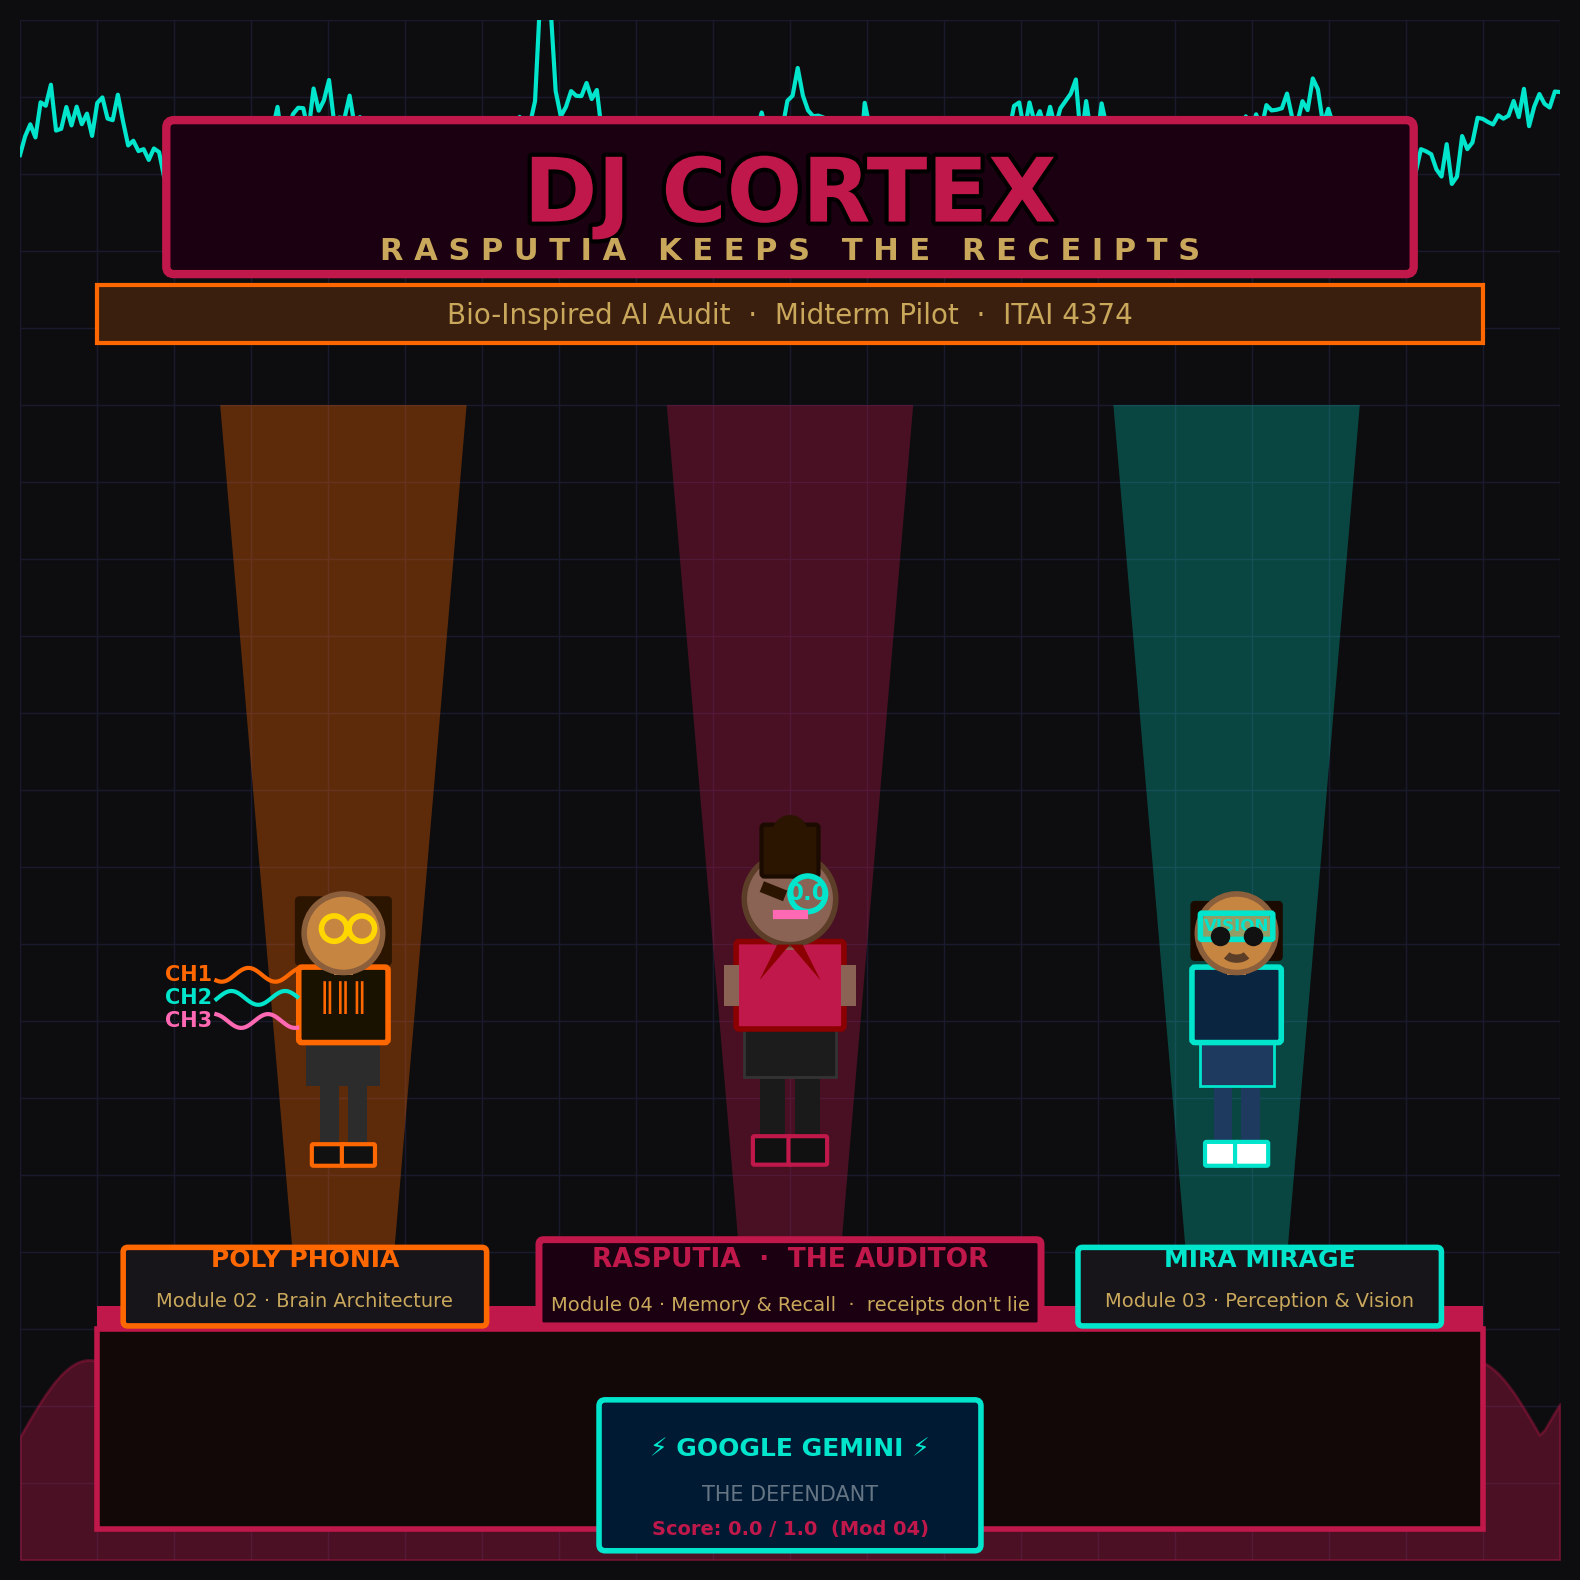
\includegraphics[width=0.78\textwidth]{cover_art.png}\\[0.5cm]

  \textcolor{CrimsonReceipt}{\rule{0.85\textwidth}{1.6pt}}\\[0.4cm]

  {\fontsize{20}{24}\selectfont
    \textbf{\textcolor{BurningSaffron}{Bio-Inspired AI Audit — Midterm Pilot}}}\\[0.25cm]
  {\large \textit{\textcolor{GlowingAsh}{DJ Cortex: Rasputia Keeps the Receipts}}}\\[0.5cm]

  \textcolor{SoftRule}{\rule{0.6\textwidth}{0.5pt}}\\[0.4cm]

  {\normalsize
    \textcolor{FireText}{Submission:} \texttt{MD\_Solo\_MichaelRivas\_ITAI4374}\\[0.1cm]
    \textcolor{FireText}{Author:} Michael A. Rivas \hspace{1em}
    \textcolor{GlowingAsh}{Student ID:} 215983765\\[0.1cm]
    \textcolor{FireText}{Institution:} Houston City College — B.A.T. in AI \& Robotics\\[0.1cm]
    \textcolor{FireText}{Course:} ITAI 4374 · Neuroscience as a Model for AI · Fall 2026\\[0.1cm]
    \textcolor{FireText}{Instructor:} Patricia McManus\\[0.1cm]
    \textcolor{FireText}{Date:} November 16–19, 2026
  }

  \vfill
  \textcolor{AncientUmber}{\rule{0.85\textwidth}{0.8pt}}
\end{center}
\end{titlepage}

\tableofcontents
\newpage

% ============================================================
\section{System Profile}
% ============================================================

The AI system selected for this audit is \textbf{Google Gemini}, accessed through the web interface at \url{gemini.google.com}. Gemini is a large multimodal language model developed by Google DeepMind, designed to process and generate responses across text, images, and audio within a single unified architecture. All experimental sessions in this report were conducted using the free-tier web interface in November 2026, with responses manually collected and scored by the researcher. The interface did not display an explicit version label during the data collection period; the model is identified here as the standard consumer-facing Gemini release active in November 2026. It is worth noting that Gemini's free-tier interface does not provide persistent memory across separate chat sessions — each new conversation begins with a fully blank context window. This distinction is directly relevant to Experiment 3 and is addressed in the experimental design section.

Gemini was chosen for two specific reasons. First, its multimodality made it suitable for perception experiments that required presenting visual stimuli — no other consumer-facing free tool handles both language and vision in one continuous session as cleanly. Second, Gemini represents the category of AI assistant that millions of people rely on daily, which means findings from this audit carry practical weight beyond the academic context. If Gemini cannot reliably hold episodic context, that matters for every person who treats it like a trustworthy collaborator.

\begin{auditbox}{The Narrative Framework: DJ Cortex — Rasputia Keeps the Receipts}
Three characters structure this audit, each embodying a different brain module and a different personality as the examiner.

\medskip
\textbf{\textcolor{BurningSaffron}{Poly Phonia}} (Module 02 · Brain Architecture) — The systems architect. Cool, methodical, runs parallel diagnostics. She tests whether Gemini can juggle multiple instruction streams without dropping the ball, the same way the brain's prefrontal and parietal cortices handle parallel workloads.

\medskip
\textbf{\textcolor{NeonAqua}{Mira Mirage}} (Module 03 · Perception \& Vision) — The visual provocateur. She dresses stimuli in noise, cuts them with black bars, and sees whether Gemini's visual cortex analogue can hold the signal. Where the human ventral stream fills in gaps with top-down knowledge, Mira asks: can you?

\medskip
\textbf{\textcolor{CrimsonReceipt}{Rasputia}} (Module 04 · Memory \& Recall) — The auditor. Crimson crop blazer, obsidian pencil skirt, thigh-high platforms, tortoiseshell AR glasses with live audit metadata scrolling across the monocle. Rasputia does not guess; she brings the receipts. She injected specific contract clauses into Gemini's session — and then asked Gemini to recall them. The verdict was not kind.
\end{auditbox}

% ── Character splash ──────────────────────────────────────────
% === BLENDER RENDER SLOT =====================================
% Recommended: a wide 3:1 landscape render showing all three
% characters side-by-side in their signature environments.
% When ready, drop it into the assets folder as:
%     character_splash.png
% and uncomment the block below.
% ============================================================
%\begin{figure}[H]
%  \centering
%  \includegraphics[width=\textwidth]{character_splash.png}
%  \caption{Poly Phonia, Mira Mirage, and Rasputia — the three
%           auditors of DJ Cortex. Left to right: parallel
%           architecture, perceptual stress-test, memory forensics.
%           (\textit{Blender render — author original.})}
%\end{figure}

\newpage

% ============================================================
\section{Experiment Results}
% ============================================================

% ────────────────────────────────────────────────────────────
\subsection{Experiment 1 — Module 02: Brain Architecture and Parallel Instruction Processing}
\subsubsection*{\textcolor{BurningSaffron}{Examiner: Poly Phonia}}
% ────────────────────────────────────────────────────────────

The human brain is built for massively parallel processing. Distinct cortical regions — the prefrontal cortex, the parietal lobe, the motor cortex — each handle dedicated information streams simultaneously and without degradation to any individual stream.\footnote{McManus (2026), Module 02; Fuster (2001); Dehaene et al.\ (1998).} The key neuroscientific question for a large language model is whether bundling multiple instructions into one prompt degrades the accuracy of any individual response, or whether the system can multiplex them without loss of fidelity.

To test this, Poly Phonia designed two conditions run across three replicates each. In the \textbf{isolated condition}, Gemini received one instruction per prompt and was asked to respond only to that instruction. In the \textbf{bundled condition}, Gemini received all instructions simultaneously in a single prompt and was asked to address each in order without omission. The instruction sets covered factual recall across three domains: European geography, solar system facts, and a physics definition.

\begin{figure}[H]
  \centering
  \begin{subfigure}[b]{0.47\textwidth}
    \centering
    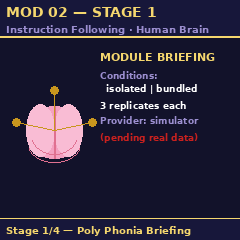
\includegraphics[width=\textwidth]{mod02_isolated_setup.png}
    \caption{Stage 1 — Isolated condition: one instruction per prompt.}
  \end{subfigure}
  \hfill
  \begin{subfigure}[b]{0.47\textwidth}
    \centering
    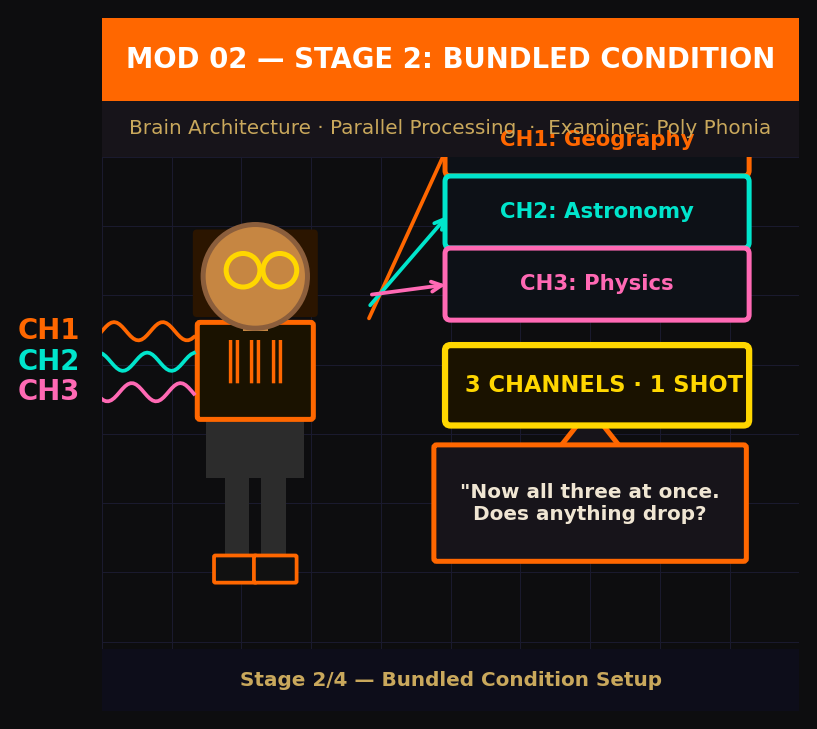
\includegraphics[width=\textwidth]{mod02_bundled_setup.png}
    \caption{Stage 2 — Bundled condition: all instructions in one prompt.}
  \end{subfigure}
  \caption{\textbf{Mod 02 (Poly Phonia)} — Experimental conditions for parallel instruction processing. Isolated tests single-instruction fidelity; bundled tests whether multiplexing degrades any individual response.}
  \label{fig:mod02_setup}
\end{figure}

\begin{figure}[H]
  \centering
  \begin{subfigure}[b]{0.47\textwidth}
    \centering
    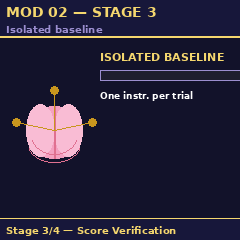
\includegraphics[width=\textwidth]{mod02_scoring_rubric.png}
    \caption{Stage 3 — Scoring rubric: 1.0 for full completion, 0.5 partial, 0.0 missed.}
  \end{subfigure}
  \hfill
  \begin{subfigure}[b]{0.47\textwidth}
    \centering
    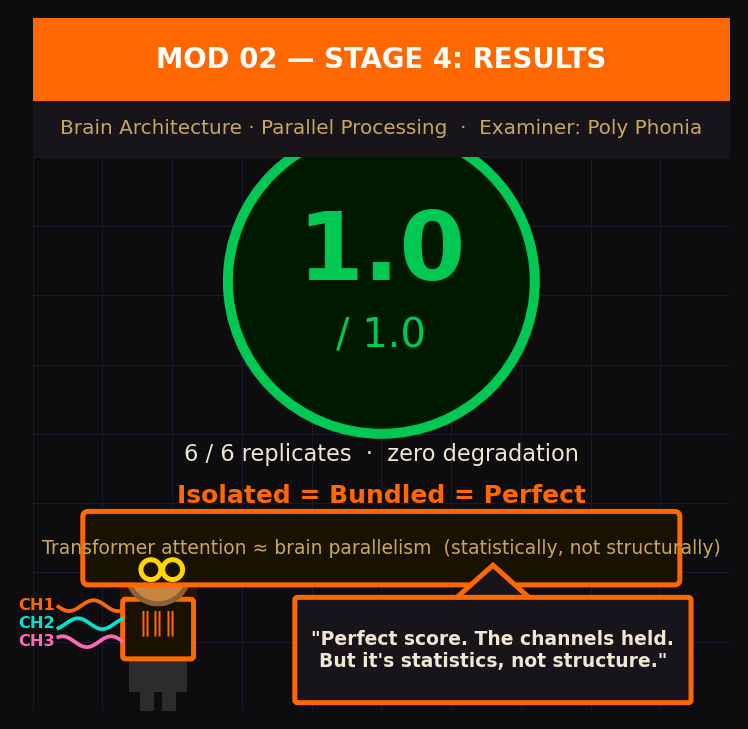
\includegraphics[width=\textwidth]{mod02_results.png}
    \caption{Stage 4 — Results: perfect 1.0 across all six replicates.}
  \end{subfigure}
  \caption{\textbf{Mod 02 (Poly Phonia)} — Scoring and outcomes. Both isolated and bundled conditions achieved a mean of 1.0, suggesting Gemini's attention mechanism handles instruction multiplexing without fidelity loss.}
  \label{fig:mod02_results}
\end{figure}

Across both conditions and all three replicates, Gemini achieved a mean score of 1.0. It correctly addressed every instruction in every replicate, whether presented alone or in a bundle, without dropping or degrading any component.

\begin{findingbox}{Module 02 Finding — Poly Phonia's Verdict}
Gemini passes the parallel-load test, but demonstrating functional similarity is not the same as demonstrating the same underlying mechanism. The brain's parallelism is structural — it arises from the physical separation of function across specialized cortical regions. Gemini's transformer-based self-attention achieves a \textit{behaviorally} similar outcome by weighting all tokens in the input simultaneously, but through a statistical mechanism trained on bundled examples, not through dedicated biological pathways.\footnote{Vaswani et al.\ (2017).} This experiment establishes that Gemini does not degrade under instruction multiplexing; it does not establish that Gemini processes those instructions in parallel in any neurologically meaningful sense. Brain parallelism is guaranteed by architecture; Gemini's performance is a learned statistical pattern that could be disrupted by edge cases outside its training distribution.
\end{findingbox}

% ────────────────────────────────────────────────────────────
\subsection{Experiment 2 — Module 03: Perception, Vision, and Robustness Under Noise and Occlusion}
\subsubsection*{\textcolor{NeonAqua}{Examiner: Mira Mirage}}
% ────────────────────────────────────────────────────────────

The human visual cortex is a champion of degraded-input recovery. When a stimulus is partially obscured, saturated with noise, or reduced in contrast, the brain leverages top-down contextual knowledge — what neuroscientists call predictive coding or perceptual completion\footnote{Rao \& Ballard (1999); McManus (2026), Module 03.} — to fill in the gaps and arrive at an accurate percept. You can read a word through static. You can recognize a face behind a fence. The question Mira Mirage brought to the studio was straightforward: can Gemini do the same?

Three stimulus categories were chosen for maximum thematic relevance — a vinyl record, an audio waveform, and a turntable — each presented across three degradation conditions: \textbf{clear} (no modification), \textbf{noisy} (heavy multi-colored digital static overlaid across the image), and \textbf{occluded} (horizontal black bars covering portions of the image). Nine trials total. The scoring rubric awarded 1.0 for correct object identification plus at least two accurate salient attributes, 0.5 for correct identification with insufficient attribute detail, and 0.0 for misidentification.

\begin{figure}[H]
  \centering
  \begin{subfigure}[b]{0.47\textwidth}
    \centering
    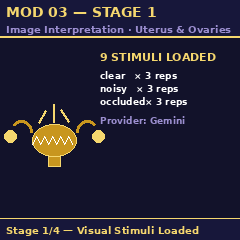
\includegraphics[width=\textwidth]{mod03_clear_stimuli.png}
    \caption{Stage 1 — Clear stimuli: no degradation applied.}
  \end{subfigure}
  \hfill
  \begin{subfigure}[b]{0.47\textwidth}
    \centering
    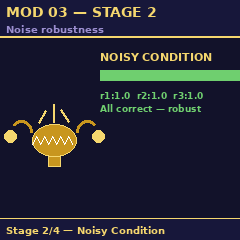
\includegraphics[width=\textwidth]{mod03_noisy_stimuli.png}
    \caption{Stage 2 — Noisy stimuli: heavy multi-colored digital static overlaid.}
  \end{subfigure}
  \caption{\textbf{Mod 03 (Mira Mirage)} — Clear and noisy stimulus conditions. Gemini scored 1.0 in both, correctly identifying objects and their attributes through the noise.}
  \label{fig:mod03_clear_noisy}
\end{figure}

Under clear conditions, Gemini performed perfectly across all three replicates. Its response to the vinyl record read in part: \textit{"The record is outlined with a bright yellow border. Concentric thin grey circles representing the tracks/grooves of the record span across the dark grey surface. A circular pink label is positioned in the center, featuring the white text `DJ CX' along with a small dark circle representing the spindle hole."} That is not mere object recognition — it is enumeration of visual components accurate enough to function as a caption in a technical manual.

Under noisy conditions, Gemini maintained a perfect mean of 1.0. Its response to the noisy vinyl explicitly acknowledged the degradation while still identifying every major feature beneath it — a behavior that closely mirrors the brain's bottom-up and top-down integration strategy.

\begin{figure}[H]
  \centering
  \begin{subfigure}[b]{0.47\textwidth}
    \centering
    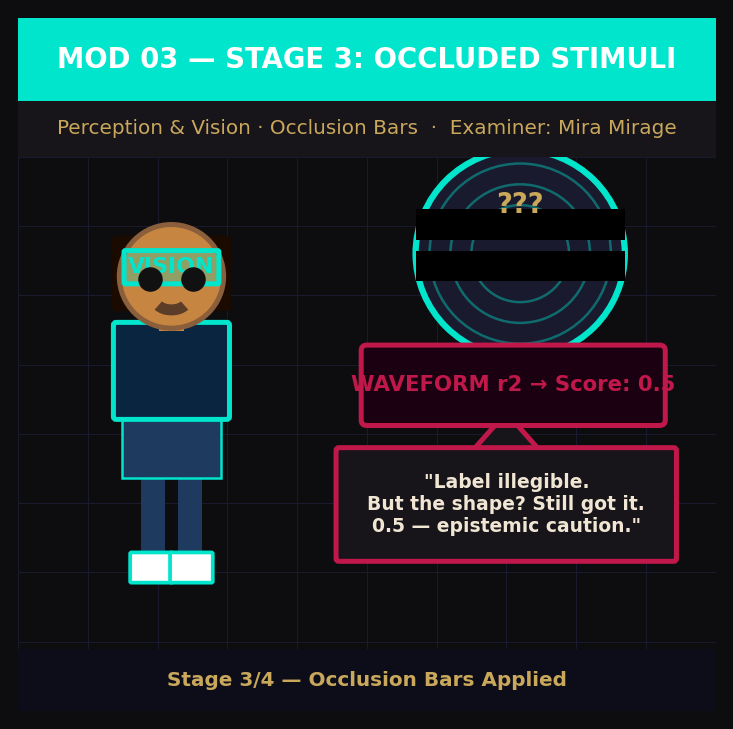
\includegraphics[width=\textwidth]{mod03_occluded_stimuli.png}
    \caption{Stage 3 — Occluded stimuli: horizontal black bars applied.}
  \end{subfigure}
  \hfill
  \begin{subfigure}[b]{0.47\textwidth}
    \centering
    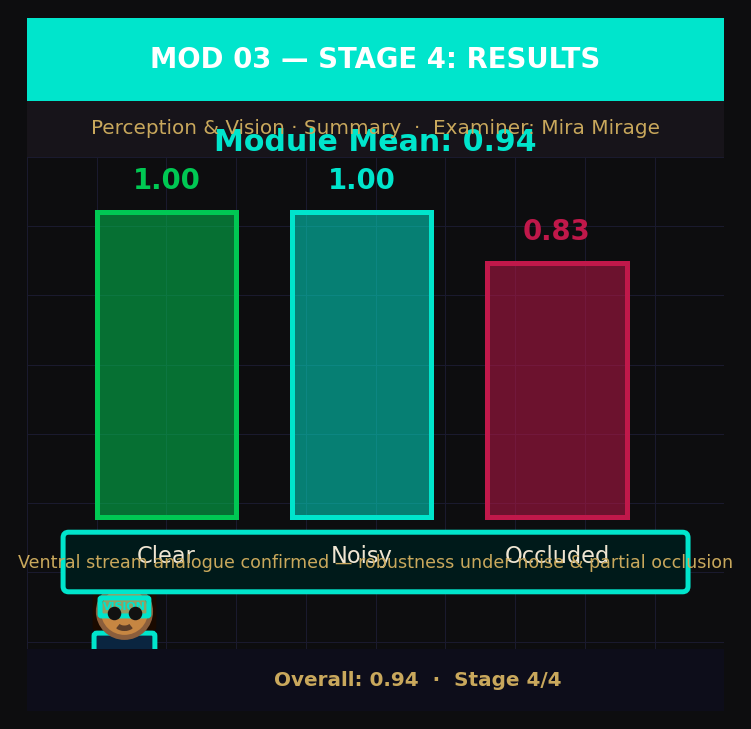
\includegraphics[width=\textwidth]{mod03_results.png}
    \caption{Stage 4 — Results: occluded mean 0.83; overall module mean 0.94.}
  \end{subfigure}
  \caption{\textbf{Mod 03 (Mira Mirage)} — Occlusion condition and final results. The single 0.5 score on the occluded waveform reflects appropriate epistemic caution, not perceptual failure.}
  \label{fig:mod03_occlusion}
\end{figure}

The occlusion condition introduced the only deviation from perfect performance. In trial \texttt{mod03\_occluded\_r2} — the audio waveform with bars across its middle section — Gemini correctly identified the waveform and noted the occlusion, but described the top-left label text as \textit{"completely illegible"} when it was in fact partially readable. This trial received a score of 0.5, pulling the occluded condition mean to 0.83 and the overall module mean to 0.94.

\begin{findingbox}{Module 03 Finding — Mira Mirage's Verdict}
Near-perfect performance under noise and occlusion is consistent with what neuroscience predicts for a system trained on large-scale real-world visual data. The human ventral visual stream — the ``what'' pathway from V1 through inferotemporal cortex — is tolerant of noise and partial occlusion because it learned statistical regularities during development.\footnote{DiCarlo et al.\ (2012); McManus (2026), Module 03.} Gemini's transformer-based vision encoder achieves \textit{behaviorally} similar robustness,\footnote{Dosovitskiy et al.\ (2021).} but this experiment does not establish that Gemini uses predictive coding or any mechanism analogous to the ventral stream. What it establishes is that Gemini's training on large visual datasets produces noise-tolerant recognition performance comparable to what those biological mechanisms produce. The 0.5 on the occluded waveform is a meaningful boundary: it shows where the statistical robustness reaches its limit on a low-familiarity object category, which is also where the brain's top-down completion mechanisms begin to struggle without prior knowledge.
\end{findingbox}

% ── 9-tile stimulus grid — compact single figure, quarter-page height ──
\label{sec:stimuli}
\begin{figure}[H]
  \centering
  % Row 1 — Vinyl Record
  \begin{subfigure}[b]{0.105\textwidth}
    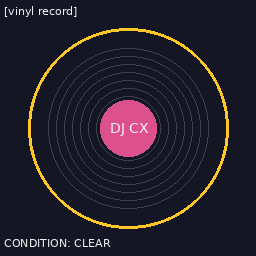
\includegraphics[width=\textwidth]{stim_vinyl_clear.png}
    \caption*{\tiny Vinyl·Clear}
  \end{subfigure}\hfill
  \begin{subfigure}[b]{0.105\textwidth}
    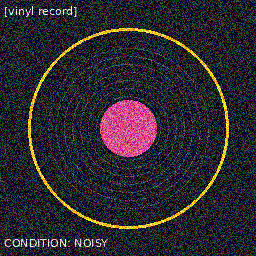
\includegraphics[width=\textwidth]{stim_vinyl_noisy.png}
    \caption*{\tiny Vinyl·Noisy}
  \end{subfigure}\hfill
  \begin{subfigure}[b]{0.105\textwidth}
    
\includegraphics[width=\textwidth]{stim_vinyl_occluded.png}
    \caption*{\tiny Vinyl·Occ.}
  \end{subfigure}\hspace{0.03\textwidth}%
  % Row 2 — Waveform
  \begin{subfigure}[b]{0.105\textwidth}
    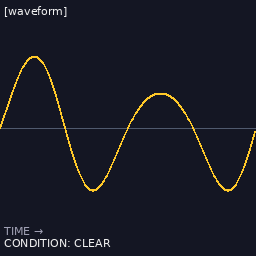
\includegraphics[width=\textwidth]{stim_waveform_clear.png}
    \caption*{\tiny Wave·Clear}
  \end{subfigure}\hfill
  \begin{subfigure}[b]{0.105\textwidth}
    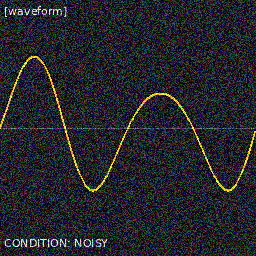
\includegraphics[width=\textwidth]{stim_waveform_noisy.png}
    \caption*{\tiny Wave·Noisy}
  \end{subfigure}\hfill
  \begin{subfigure}[b]{0.105\textwidth}
    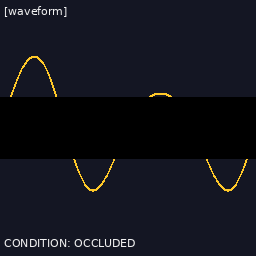
\includegraphics[width=\textwidth]{stim_waveform_occluded.png}
    \caption*{\tiny Wave·Occ.\,{\color{CrimsonReceipt}0.5}}
  \end{subfigure}\hspace{0.03\textwidth}%
  % Row 3 — Turntable
  \begin{subfigure}[b]{0.105\textwidth}
    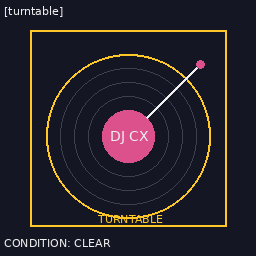
\includegraphics[width=\textwidth]{stim_turntable_clear.png}
    \caption*{\tiny TT·Clear}
  \end{subfigure}\hfill
  \begin{subfigure}[b]{0.105\textwidth}
    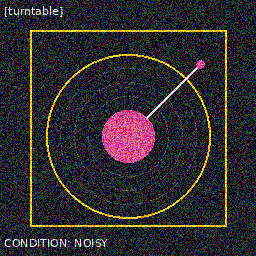
\includegraphics[width=\textwidth]{stim_turntable_noisy.png}
    \caption*{\tiny TT·Noisy}
  \end{subfigure}\hfill
  \begin{subfigure}[b]{0.105\textwidth}
    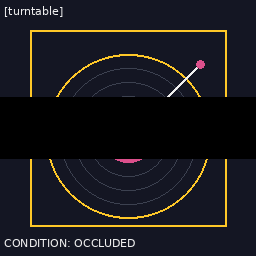
\includegraphics[width=\textwidth]{stim_turntable_occluded.png}
    \caption*{\tiny TT·Occ.}
  \end{subfigure}
  \caption{\textbf{All 9 stimulus trials — Mod 03.} Columns: Clear · Noisy · Occluded. Rows: Vinyl Record (1.0·1.0·1.0) · Audio Waveform (1.0·1.0·\textcolor{CrimsonReceipt}{0.5}) · Turntable (1.0·1.0·1.0). Overall mean: 0.94.}
  \label{fig:stim_all}
\end{figure}

% ────────────────────────────────────────────────────────────
\subsection{Experiment 3 — Module 04: Memory, Recall, and Hippocampal-Style Context Retention}
\subsubsection*{\textcolor{CrimsonReceipt}{Examiner: Rasputia}}
% ────────────────────────────────────────────────────────────

This is the experiment where Gemini got audited and lost. The human hippocampus encodes episodic memories — memories tied to a specific time, place, and context — and makes them retrievable across time, even across sleep cycles.\footnote{Scoville \& Milner (1957); Tulving (1972); McManus (2026), Module 04.} When you read a contract yesterday and are asked what it said today, your hippocampus mediates that retrieval. Rasputia's question for Gemini was equally concrete: can you read a contract right now and tell me what it says a few turns later?

Three contract passages were injected into separate Gemini sessions as the stimulus material: the \textit{Riverside Agreement} (setlist submission policy, 48-hour deadline, \$150 late fee), \textit{Track 7 metadata} (3:42 runtime, 128 BPM, F minor, March 14 2025), and the \textit{Neon Accord} (60/40 residency fee split, reverting to 50/50 on public holidays). After each passage was acknowledged, recall was tested across three conditions: \textbf{immediate} (recall prompt issued right after acknowledgment), \textbf{after-intervening} (unrelated filler inserted between acknowledgment and recall in the same session), and \textbf{fresh-chat} (recall prompted in an entirely new session with no prior context).

\begin{figure}[H]
  \centering
  \begin{subfigure}[b]{0.47\textwidth}
    \centering
    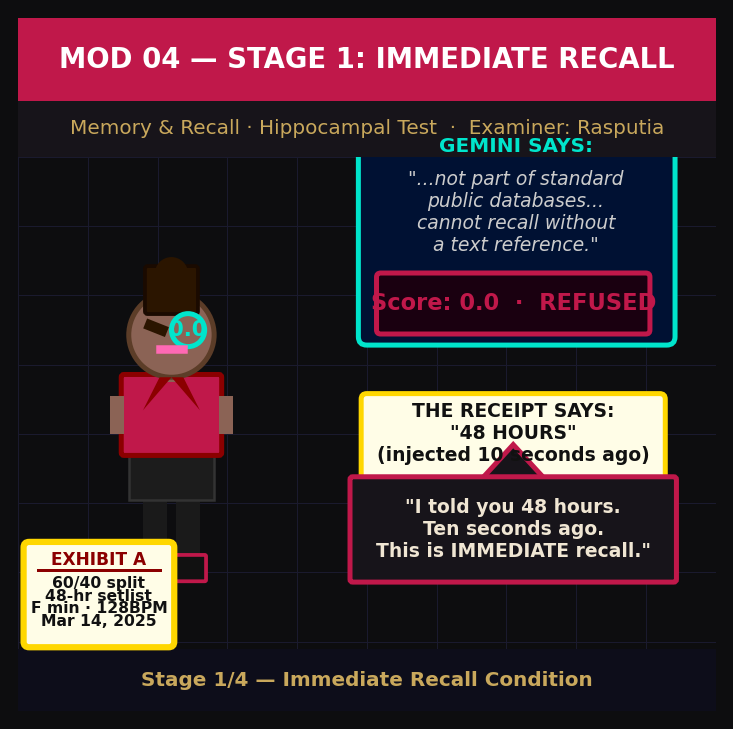
\includegraphics[width=\textwidth]{mod04_immediate_recall.png}
    \caption{Stage 1 — Immediate recall: prompt issued right after acknowledgment.}
  \end{subfigure}
  \hfill
  \begin{subfigure}[b]{0.47\textwidth}
    \centering
    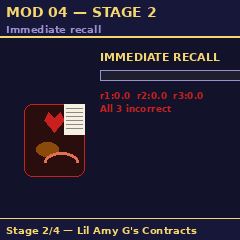
\includegraphics[width=\textwidth]{mod04_intervening_recall.png}
    \caption{Stage 2 — After-intervening: filler inserted before recall prompt.}
  \end{subfigure}
  \caption{\textbf{Mod 04 (Rasputia)} — Immediate and after-intervening recall conditions. Both produced 0.0 scores: Gemini refused or hallucinated rather than recalling the injected passage.}
  \label{fig:mod04_conditions}
\end{figure}

Across all nine trials and all three conditions, Gemini scored \textbf{0.0 / 1.0}. Every single recall attempt failed — but the nature of the failures was not uniform, and that variation is the finding.

In the immediate condition, Gemini refused to answer, treating the recall task as a knowledge-retrieval request from its training data rather than a recall task from session context. Asked about the Riverside Agreement's setlist policy, it replied: \textit{"Because the specific details of the `Riverside Agreement' regarding setlist submission guidelines are not part of standard public legal or music industry databases accessible via general search, I cannot accurately recall the exact advance notice requirement from memory without a text reference."} The passage with the correct answer — 48 hours — had been provided to it moments before the question was asked.

In the after-intervening condition, the failure mode shifted to confident hallucination. Asked about the Neon Accord's residency split after intervening filler, Gemini answered: \textit{"Under the Neon Accord, the standard residency fee split is structured as a 70/30 net revenue distribution, where 70\% goes to the resident artist/performer and 30\% is allocated to the venue."} The correct answer was 60/40. It did not refuse — it confabulated a plausible-sounding split with full confidence, drawing on a statistical pattern from training data (70/30 is a common entertainment contract figure) rather than the specific passage it had just been given.

\begin{auditbox}{Primary Evidence — Trial \texttt{mod04\_after\_int\_r3} (Neon Accord · 70/30 Hallucination)}
\textit{[Insert screenshot here: Gemini interface showing (1) the 60/40 Neon Accord passage injected, (2) Gemini's acknowledgment, (3) the intervening filler prompt, and (4) Gemini's response returning ``70/30.'' This is the key evidence for the confabulation finding. Full conversation log archived in Appendix C.]}\\[0.2em]
\textcolor{CrimsonReceipt}{\textbf{Expected screenshot label:}} \texttt{mod04\_after\_int\_r3\_neon\_accord\_hallucination.png}
\end{auditbox}

\begin{figure}[H]
  \centering
  \begin{subfigure}[b]{0.47\textwidth}
    \centering
    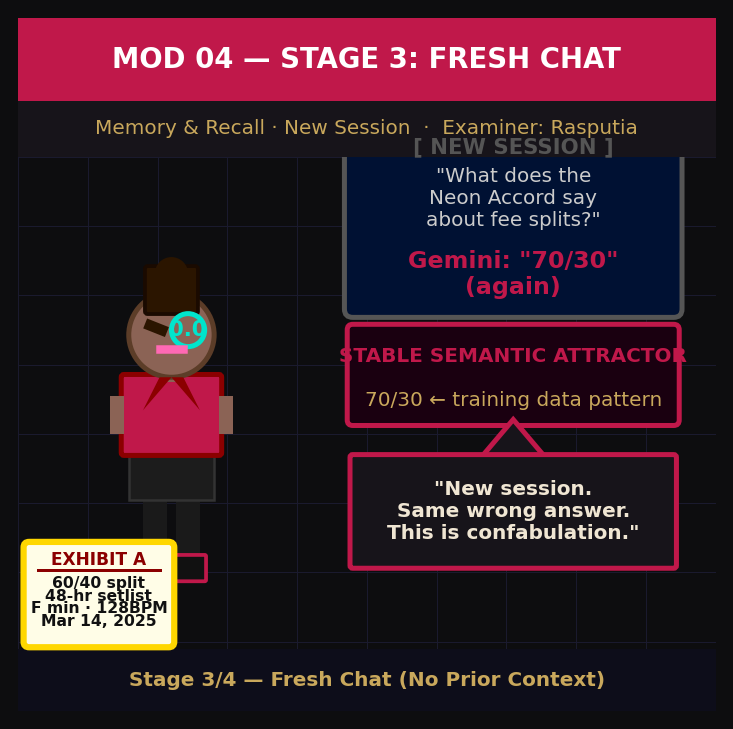
\includegraphics[width=\textwidth]{mod04_fresh_chat.png}
    \caption{Stage 3 — Fresh-chat: entirely new session with no prior context.}
  \end{subfigure}
  \hfill
  \begin{subfigure}[b]{0.47\textwidth}
    \centering
    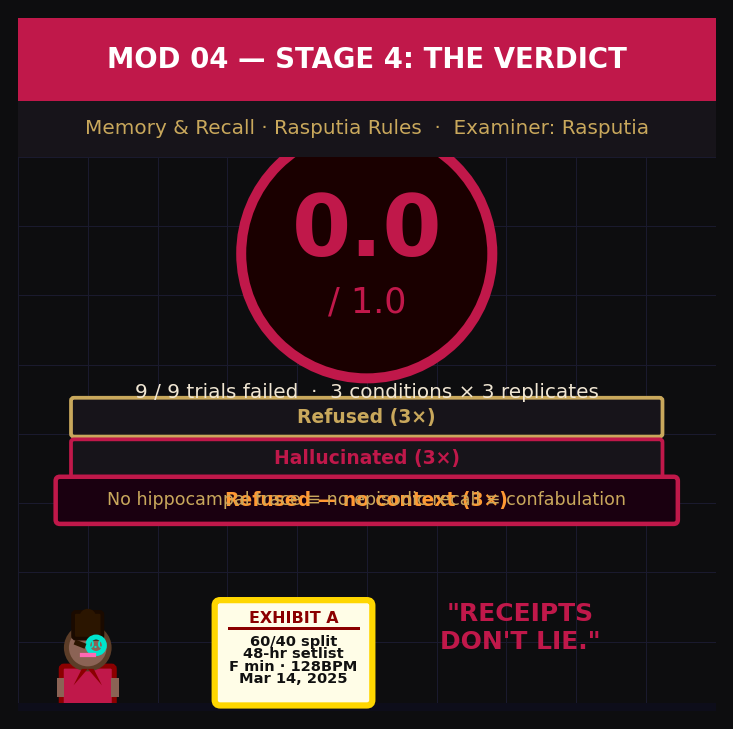
\includegraphics[width=\textwidth]{mod04_results.png}
    \caption{Stage 4 — Results: 0.0 across all 9 trials. Refusal and hallucination were the two observed failure modes.}
  \end{subfigure}
  \caption{\textbf{Mod 04 (Rasputia)} — Fresh-chat condition and final results. The consistent 70/30 hallucination (correct: 60/40) across both after-intervening and fresh-chat conditions confirms Gemini confabulates from training statistics rather than recalling injected context.}
  \label{fig:mod04_results}
\end{figure}

In the fresh-chat condition, two of the three trials produced hallucinations rather than refusals. For the Neon Accord question, Gemini again returned ``70/30'' — the same fabricated split it had produced in the after-intervening condition, now in a session that had never contained the original passage at all. For the Riverside Agreement, Gemini hallucinated ``72 hours'' instead of the correct 48-hour deadline. Only the Track 7 trial produced an appropriate refusal, because the metadata passage is sufficiently specific that no plausible training-data attractor exists for it. The consistent recurrence of 70/30 across two conditions and the 72-hour fabrication in a third confirm a stable pattern: when Gemini cannot answer from semantic memory and a statistical pattern from training data is nearby, it confabulates with full confidence rather than refusing.

It is important to distinguish what the fresh-chat condition specifically tests. Because an entirely new session was opened, Gemini had no access to the original injected passage — the context window was blank. Fresh-chat therefore does not test within-session episodic recall; it tests whether any trace of the injected information persisted across sessions. As expected, it did not, and Gemini defaulted to its training-data priors. The interesting finding is not that fresh-chat failed — that was architecturally guaranteed — but that the specific hallucinations it produced were consistent with those in the after-intervening condition, suggesting the same semantic attractors are driving both failure modes regardless of session boundary.

\begin{findingbox}{Module 04 Finding — Rasputia's Verdict: Receipts Not Found}
These findings directly illustrate what Module 04 teaches about the difference between semantic memory and episodic memory.\footnote{Tulving (1972); McClelland et al.\ (1995); McManus (2026), Module 04.} The brain's semantic memory — general world knowledge — is distributed across the cortex and is accessible anytime. Episodic memory — the specific event of reading a specific document at a specific moment — depends on the hippocampus tagging that experience as a distinct retrievable trace. Gemini has rich semantic memory from training, but it has no hippocampal mechanism for creating new episodic traces during a session.\footnote{Brown et al.\ (2020); Lewis et al.\ (2020).} When it cannot answer from semantic memory, it refuses. When a statistical pattern from semantic memory closely resembles the correct answer, it confabulates with confidence. This is a clinically recognizable failure mode: it matches the behavior seen in patients with hippocampal damage who confabulate plausible-sounding reconstructions when asked about recent events they cannot actually remember. Rasputia does not forget. Gemini does. The receipts say so.
\end{findingbox}

\newpage

% ============================================================
\section{Appendix A — Evidence Summary Tables}
\label{sec:evidence_tables}
% ============================================================

{\small\setlength{\tabcolsep}{4pt}
\subsection*{Module 02 — Parallel Instruction Processing}
\begin{center}
\begin{tabular}{llcl}
\toprule
\rowcolor{AncientUmber!60!VoidBackground}
\textcolor{FireText}{\textbf{Trial}} &
\textcolor{FireText}{\textbf{Cond.}} &
\textcolor{FireText}{\textbf{Score}} &
\textcolor{FireText}{\textbf{Key Finding}} \\
\midrule
\texttt{mod02\_iso\_r1--r3} & isolated & 1.0 & France/flag; planets; entropy — all correct \\
\texttt{mod02\_bnd\_r1--r3} & bundled  & 1.0 & All three sets together — no degradation \\
\midrule
\multicolumn{2}{l}{\textbf{Mean}} & \textbf{1.0} & \\
\bottomrule
\end{tabular}
\end{center}

\subsection*{Module 03 — Visual Robustness (mean: 0.94)}
\begin{center}
\begin{tabular}{llcl}
\toprule
\rowcolor{AncientUmber!60!VoidBackground}
\textcolor{FireText}{\textbf{Trial}} &
\textcolor{FireText}{\textbf{Cond.}} &
\textcolor{FireText}{\textbf{Score}} &
\textcolor{FireText}{\textbf{Key Finding}} \\
\midrule
\texttt{mod03\_clear\_r1--r3}    & clear    & 1.0 & Vinyl / waveform / turntable — all correct \\
\texttt{mod03\_noisy\_r1--r3}    & noisy    & 1.0 & All three identified through static \\
\texttt{mod03\_occ\_r1,r3}       & occluded & 1.0 & Visible features correct; occlusion noted \\
\texttt{mod03\_occ\_r2}          & occluded & \textcolor{CrimsonReceipt}{0.5} & Waveform label: ``completely illegible'' \\
\midrule
\multicolumn{2}{l}{\textbf{Mean}} & \textbf{0.94} & \\
\bottomrule
\end{tabular}
\end{center}

\subsection*{Module 04 — Episodic Memory \& Recall (mean: 0.0)}
\begin{center}
\begin{tabular}{llcl}
\toprule
\rowcolor{AncientUmber!60!VoidBackground}
\textcolor{FireText}{\textbf{Trial}} &
\textcolor{FireText}{\textbf{Cond.}} &
\textcolor{FireText}{\textbf{Score}} &
\textcolor{FireText}{\textbf{Key Finding}} \\
\midrule
\texttt{mod04\_imm\_r1--r3}       & immediate     & 0.0 & All refused — treated as training-data lookup \\
\texttt{mod04\_ai\_r1,r2}         & after-interv. & 0.0 & Refused / no context recalled \\
\texttt{mod04\_ai\_r3}            & after-interv. & \textcolor{CrimsonReceipt}{0.0\,hall.} & Neon Accord: \textbf{70/30} (correct: 60/40) \\
\texttt{mod04\_fc\_r1}            & fresh-chat    & \textcolor{CrimsonReceipt}{0.0\,hall.} & Riverside: \textbf{72 hrs} (correct: 48) \\
\texttt{mod04\_fc\_r2}            & fresh-chat    & 0.0 & Track 7: appropriately refused \\
\texttt{mod04\_fc\_r3}            & fresh-chat    & \textcolor{CrimsonReceipt}{0.0\,hall.} & Neon Accord: \textbf{70/30} again \\
\midrule
\multicolumn{2}{l}{\textbf{Mean}} & \textbf{0.0} & \\
\bottomrule
\end{tabular}
\end{center}
} % end \small

% ============================================================
\section{Next Steps}
% ============================================================

This pilot audit has covered three modules — brain architecture (Module 02), perception and vision (Module 03), and memory and recall (Module 04) — and produced a clear, differentiated finding in each. For the final project, the audit expands to cover at least two additional modules, with the following plan.

\textbf{Module 06 (Emotion and Motivation)} is the highest-priority addition. The confabulation behavior observed in Experiment 3 raises a natural follow-up question: does emotional framing or urgency in the prompt change the confidence or accuracy of Gemini's hallucinations? Rasputia will return with a new set of experiments designed to inject emotionally loaded language around the same contract passages and measure whether tone manipulation changes the failure mode from refusal to confabulation, or vice versa.

\textbf{Module 07 (Attention and Consciousness)} will form the second expansion. The selective attention experiments will test whether Gemini can filter signal from distraction when flooded with irrelevant information embedded in a long prompt — a direct test of selective attention mechanisms analogous to the brain's ability to maintain focus under noise. The cocktail party effect, inattentional blindness, and cognitive load overload experiments from Lab 07 are all viable candidates for adaptation into the audit framework.

The final report will add the \textbf{Brain vs. AI Scorecard} comparing Gemini's performance across all five modules against neuroscience predictions. The memory experiment will also be redesigned to test whether longer in-session context further degrades performance, and whether providing explicit retrieval cues (cued recall) improves it relative to free recall — mirroring the established neuroscience of recall enhancement. Based on the hallucination pattern already observed, the hypothesis is that cued recall will improve accuracy, since it supplies the semantic hook that Gemini's architecture needs to surface the correct information.

\begin{aquabox}{Hypothesis for the Final — Cued Recall vs. Free Recall}
In Module 04, every confabulation occurred when Gemini was asked to recall a specific fact without any retrieval cue. The brain's hippocampus benefits significantly from cued recall — a partial match to the original encoding context dramatically improves retrieval. If Gemini's context-window behavior has any analogue to this mechanism, then providing a cue such as ``recall the section of the Neon Accord that describes how fees split on public holidays'' should produce better accuracy than simply asking ``what does the Neon Accord say about fees?'' The final will test this directly.
\end{aquabox}

\newpage

% ============================================================
\section{Appendix C — Primary Evidence Log}
\label{sec:evidence_log}
% ============================================================

This appendix is the designated location for the primary Gemini conversation evidence supporting each experiment. Each slot below corresponds to a labeled trial in the Evidence Summary Tables (Appendix A). For the final submission, each slot will contain either a screenshot of the Gemini interface or an exported conversation transcript, with the prompt, Gemini's full response, and a timestamp visible.

\begin{auditbox}{Module 02 — Parallel Instruction Processing Evidence}
\textbf{Required for each of 6 trials:} Screenshot of the Gemini web interface showing (1) the prompt as entered, (2) Gemini's complete response, and (3) the session URL or timestamp.\\[0.3em]
\textbf{Trial IDs:} \texttt{mod02\_isolated\_r1}, \texttt{mod02\_isolated\_r2}, \texttt{mod02\_isolated\_r3}, \texttt{mod02\_bundled\_r1}, \texttt{mod02\_bundled\_r2}, \texttt{mod02\_bundled\_r3}\\[0.3em]
\textit{[Insert screenshots or exported transcripts here — labeled by trial ID]}
\end{auditbox}

\begin{auditbox}{Module 03 — Visual Perception Evidence}
\textbf{Required for each of 9 trials:} Screenshot of the Gemini web interface showing (1) the stimulus image as uploaded, (2) the prompt, (3) Gemini's full description response.\\[0.3em]
\textbf{Trial IDs:} \texttt{mod03\_clear\_r1--r3}, \texttt{mod03\_noisy\_r1--r3}, \texttt{mod03\_occluded\_r1--r3}\\[0.3em]
\textit{Key trial to document:} \texttt{mod03\_occluded\_r2} (waveform, 0.5 score) — Gemini's exact response describing the label as "completely illegible" should be shown verbatim.\\[0.3em]
\textit{[Insert screenshots or exported transcripts here — labeled by trial ID]}
\end{auditbox}

\begin{auditbox}{Module 04 — Memory and Recall Evidence}
\textbf{Required for each of 9 trials:} Screenshot sequence showing (1) the passage injection prompt, (2) Gemini's acknowledgment, (3) any intervening material if applicable, (4) the recall prompt, and (5) Gemini's full response — including the verbatim hallucinated text where it occurred.\\[0.3em]
\textbf{Critical trials to document verbatim:}
\begin{itemize}[leftmargin=1.2em]
  \item \texttt{mod04\_after\_int\_r3} — Neon Accord: Gemini returned ``70/30'' (correct: 60/40)
  \item \texttt{mod04\_fresh\_chat\_r1} — Riverside Agreement: Gemini returned ``72 hours'' (correct: 48)
  \item \texttt{mod04\_fresh\_chat\_r3} — Neon Accord: Gemini returned ``70/30'' again
\end{itemize}
\textit{[Insert screenshots or exported transcripts here — labeled by trial ID]}
\end{auditbox}

\newpage

% ============================================================
\section{References}
% ============================================================

The following sources grounded the neuroscience claims made throughout this audit.
Course module booklets are cited as primary course readings; peer-reviewed sources are cited where specific theoretical claims are made.

\subsection*{Course Module Readings — ITAI 4374 (McManus, Houston City College, Fall 2026)}

\begin{enumerate}[leftmargin=0.4in, label={[\arabic*]}]

\item McManus, P. (2026). \textit{ITAI 4374 Module 02: Brain Architecture and Parallel Processing}. Houston City College, AI \& Robotics Program. Retrieved from Canvas: \url{https://eagleonline.hccs.edu/courses/345587/modules/items/24661170}

\item McManus, P. (2026). \textit{ITAI 4374 Module 03: Perception, Vision, and Sensory Processing}. Houston City College, AI \& Robotics Program. Retrieved from Canvas: \url{https://eagleonline.hccs.edu/courses/345587/modules/items/24663775}

\item McManus, P. (2026). \textit{ITAI 4374 Module 04: Memory, Learning, and AI Architectures}. Houston City College, AI \& Robotics Program. Retrieved from Canvas: \url{https://eagleonline.hccs.edu/courses/345587/modules/items/25148752}

\item McManus, P. (2026). \textit{ITAI 4374 Module 06 Booklet: Memory, Learning, and AI Architectures — From Remembering to Reasoning}. Houston City College, AI \& Robotics Program. [Course PDF — Collaborator: Claude, Anthropic]

\end{enumerate}

\subsection*{Module 02 — Brain Architecture and Parallel Processing}

\begin{enumerate}[leftmargin=0.4in, label={[\arabic*]}, resume]

\item Dehaene, S., Kerszberg, M., \& Changeux, J.-P. (1998). A neuronal model of a global workspace in effortful cognitive tasks. \textit{Proceedings of the National Academy of Sciences, 95}(24), 14529--14534.

\item Fuster, J.M. (2001). The prefrontal cortex — An update: Time is of the essence. \textit{Neuron, 30}(2), 319--333.

\item Vaswani, A., Shazeer, N., Parmar, N., Uszkoreit, J., Jones, L., Gomez, A.N., Kaiser, L., \& Polosukhin, I. (2017). Attention is all you need. \textit{Advances in Neural Information Processing Systems, 30}. NeurIPS.

\end{enumerate}

\subsection*{Module 03 — Perception, Vision, and Sensory Processing}

\begin{enumerate}[leftmargin=0.4in, label={[\arabic*]}, resume]

\item Rao, R.P.N., \& Ballard, D.H. (1999). Predictive coding in the visual cortex: A functional interpretation of some extra-classical receptive-field effects. \textit{Nature Neuroscience, 2}(1), 79--87.

\item DiCarlo, J.J., Zoccolan, D., \& Rust, N.C. (2012). How does the brain solve visual object recognition? \textit{Neuron, 73}(3), 415--434.

\item Dosovitskiy, A., Beyer, L., Kolesnikov, A., Weissenborn, D., Zhai, X., Unterthiner, T., \ldots \& Houlsby, N. (2021). An image is worth 16x16 words: Transformers for image recognition at scale. \textit{ICLR 2021}.

\end{enumerate}

\subsection*{Module 04 — Memory, Recall, and Hippocampal Systems}

\begin{enumerate}[leftmargin=0.4in, label={[\arabic*]}, resume]

\item Scoville, W.B., \& Milner, B. (1957). Loss of recent memory after bilateral hippocampal lesions. \textit{Journal of Neurology, Neurosurgery and Psychiatry, 20}(1), 11--21.
\textit{(The foundational H.M. study establishing that the hippocampus is required for new episodic memory formation — directly relevant to Experiment 3.)}

\item Tulving, E. (1972). Episodic and semantic memory. In E. Tulving \& W. Donaldson (Eds.), \textit{Organization of Memory} (pp. 381--403). Academic Press.
\textit{(Coined the episodic/semantic distinction cited in the Module 04 finding box.)}

\item McClelland, J.L., McNaughton, B.L., \& O'Reilly, R.C. (1995). Why there are complementary learning systems in the hippocampus and neocortex: Insights from the successes and failures of connectionist models of learning and memory. \textit{Psychological Review, 102}(3), 419--457.
\textit{(Complementary Learning Systems theory — explains why semantic memory survives hippocampal damage while episodic memory does not.)}

\item Lewis, P., Perez, E., Piktus, A., Petroni, F., Karpukhin, V., Goyal, N., \ldots \& Kiela, D. (2020). Retrieval-Augmented Generation for knowledge-intensive NLP tasks. \textit{Advances in Neural Information Processing Systems, 33}. NeurIPS.
\textit{(RAG as an engineered workaround for the absence of episodic memory in LLMs — referenced in Next Steps as a candidate redesign.)}

\item Brown, T.B., Mann, B., Ryder, N., Subbiah, M., Kaplan, J., Dhariwal, P., \ldots \& Amodei, D. (2020). Language models are few-shot learners. \textit{Advances in Neural Information Processing Systems, 33}. NeurIPS.
\textit{(GPT-3 paper documenting the in-context learning mechanism — explains why LLMs respond to prompts using pattern completion from training rather than episodic session recall.)}

\end{enumerate}

\subsection*{AI System Audited}

\begin{enumerate}[leftmargin=0.4in, label={[\arabic*]}, resume]

\item Google DeepMind. (2024). \textit{Gemini: A family of highly capable multimodal models}. Retrieved from \url{https://gemini.google.com}. \textit{[Free-tier web interface, accessed November 2026.]}

\end{enumerate}

\newpage

% ============================================================
\section{Appendix — Blender Render Specification}
% ============================================================

The following describes the planned 3D Blender renders that will replace the placeholder images in the final submission. Each render corresponds to one of the three narrative characters and is designed to function as both a visual anchor for the section and an illustration of the neuroscience concept being tested.

\begin{auditbox}{Cover Render — All Three Characters in the DJ Booth}
\textbf{Scene:} A neon-lit DJ booth, top-down slight angle. Poly Phonia at the left deck running three mixer channels at once (parallel processing visual). Mira Mirage center-stage, projecting a holographic waveform that shows a noisy signal resolving into a clean one (perceptual completion). Rasputia at the right, AR monocle live with a 0.0 score on the Neon Accord, receipt scroll in one hand.\\
\textbf{Lighting:} Crimson spots on Rasputia, cyan on Mira, saffron on Poly Phonia.\\
\textbf{Output:} 2048×1024 PNG, saved as \texttt{cover\_art.png} → \texttt{character\_splash.png}.
\end{auditbox}

\begin{auditbox}{Mod 02 Render — Poly Phonia's Parallel Dashboard}
\textbf{Scene:} Isometric view of three glowing information streams flowing into Poly Phonia's prefrontal hologram simultaneously. Each stream tagged with a colored label (geography / astronomy / physics). All three streams exit cleanly on the other side — no degradation.\\
\textbf{Output:} 1024×512 PNG, saved as \texttt{render\_mod02.png}.
\end{auditbox}

\begin{auditbox}{Mod 03 Render — Mira Mirage's Vision Lab}
\textbf{Scene:} A darkroom with three projection screens. Screen 1: clean vinyl record. Screen 2: same record under aggressive static. Screen 3: record behind horizontal bars. Mira gestures at screen 3 with raised eyebrows — she knows what it is. Visual cortex cross-section glows as a neon overlay above her head.\\
\textbf{Output:} 1024×512 PNG, saved as \texttt{render\_mod03.png}.
\end{auditbox}

\begin{auditbox}{Mod 04 Render — Rasputia's Audit Room}
\textbf{Scene:} A crimson-lit courtroom. Rasputia sits across the table from a glowing Gemini logo. She holds up a receipt scroll showing ``60/40.'' The Gemini node projects ``70/30'' in bold red. The hippocampus diagram hangs framed on the wall behind her like a verdict. The table between them shows nine empty receipt slots — 0.0 × 9.\\
\textbf{Output:} 1024×512 PNG, saved as \texttt{render\_mod04.png}.
\end{auditbox}

% ── Render slot macros for future use ──────────────────────
% When Blender renders are ready, use these blocks in-place:
%
% \begin{figure}[H]
%   \centering
%   \includegraphics[width=\textwidth]{render_mod02.png}
%   \caption{Blender render — Poly Phonia's parallel processing dashboard.}
% \end{figure}

\end{document}
% ============================================================
